\section{Lab Four: Finding Syntactic Bugs}

\texttt{Linting} is the process of finding \textit{syntactic} problems in code.
For example, any use of the function \verb|strcpy()| is now considered unsafe
and should be replaced with a more robust string copy method. 
Searching for uses of this function is linting.

Infer has a robust linting capability. It uses a domain specific language
called "AL" which is very advanced. We are only going to cover the surface 
of what you can do with AL. In particular, you should look at the fairly
extensive documentation on AL here: \verb|https://fbinfer.com/docs/linters.html|
and at the linters that come with Infer by default - from the root of the Infer installation  
find them as follows:  \verb|find . -name "*.al"|.

\subsection{Creating a linter: Part One}

In this section we are going to create a very simple linter using AL 
to find the unsafe functions \verb|atoi()| and \verb|strcpy()|. 
These are just to obvious choices of potentially many functions you would want to audit.

\begin{itemize}
	\item Create the following file: \verb|mylinter.al|
	\item Add the following content: we will go through what this means presently.
	\begin{verbatim}
DEFINE-CHECKER UNSAFE_FUNCTION_USAGE = {
	LET isatoi = call_function(REGEXP("\\batoi"));
	SET report_when =
		isatoi;
	SET message = "Unsafe function usage - atoi()";
	SET suggestion = "See Reference - TODO";
	SET severity = "ERROR";
};

DEFINE-CHECKER UNSAFE_FUNCTION_USAGE = {
	LET isstrcpy = call_function(REGEXP("\\bstrcpy"));
	SET report_when =
		isstrcpy;
	SET message = "Unsafe function usage - strcpy()";
	SET suggestion = "See Reference - TODO";
	SET severity = "ERROR";
};
	\end{verbatim}
	\item For each of the targets, run Infer as follows using the command below.\\
	Remember to \verb|make clean| and remove any prior \verb|infer-out| directory.\\
	\verb|# infer run --keep-going --linters-only --linters-def-file mylinter.al -- make|
\end{itemize}

You should see something like the following:

\begin{verbatim}
...
Summary of the reports

UNSAFE_FUNCTION_USAGE: 21
\end{verbatim}

Create a HTML report and have look at some of the traces.

\subsection{Understanding AL}

AL is a pattern matching language that operates on Clang's \textit{Abstract Syntax Tree} (AST).
The type of pattern matching is called \textit{Computational Tree Logic} (CTL).
CTL is a way of specifying pattern matching on tree structures. 
See "AL Formulas" at \verb|https://fbinfer.com/docs/linters.html| for a detailed 
description of how to do this.

The AST is a tree of the syntactic structure of the compiled source code produced by Clang.
Therefore we need to specify the syntactic pattern we are interested in finding in the AST
in terms of AL formulas. We will look at this in a moment.

Linting in AL consists of specifying one or more checkers. 
A checker consists of
\begin{itemize}
	\item One or more \textbf{formulas} that are triggered by a syntactic pattern in the AST;
	\item A \textbf{report rule} which causes a bug report to be raised. 
	The report rule consists of a combination of formulas that when true trigger the report;
	\item A \textbf{message} which summarises the issue;
	\item A \textbf{suggestion} of what to do about the issue;
	\item A \textbf{severity} to indicate how serious the issue is.
\end{itemize}

Lets analyse the following:

\begin{verbatim}
DEFINE-CHECKER UNSAFE_FUNCTION_USAGE = {
	LET isstrcpy = call_function(REGEXP("\\bstrcpy"));
	SET report_when =
		isstrcpy;
	SET message = "Unsafe function usage - strcpy()";
	SET suggestion = "See Reference - TODO";
	SET severity = "ERROR";
};
\end{verbatim}

Observe the following:
\begin{itemize}
	\itemsep0em
	\item We create the checker \verb|UNSAFE_FUNCTION_USAGE|
	\item We create a simple formula \verb|isstrcpy|
	\item We specify an AST pattern using \verb|call_function| which matches Clang's AST node for function call sites;
	\item We further specify a regex for function names which in our case matches \verb|strcpy|
	\item We specify a report to be raised when the \verb|isstrcpy| formulae is satisfied;
	\item The remaining lines are straight forward
\end{itemize}

This example demonstrates the basic structure of a linting checker. 
We will now look at a more involved example.

\subsection{Creating a Linter: Part Two}

In this section you will create a linter for the ``unsafe pointer accumulation 
using \verb|snprintf()|'' bug. Consider the following code:

\begin{verbatim}
#include <stdio.h>
#include <string.h>
#include <stdlib.h>
#include <stdbool.h>
    
#define SIZE 1024
    
/* Snippet to demonstrate the snprintf() pointer accumulation bug */
int main(int argc, char** argv) {
    char* buf = malloc(SIZE);
    char* text = NULL;
    char* q = text; //indexing ptr into text
    size_t len = 0; //of bytes written to buf 
    size_t tlen = 0; //length on source text
    
    text = malloc(SIZE);
    strcpy(text, "the quick brown fox jumped over the lazy dog");
    q = text;
    tlen = strlen(text);
    bool islast = false;
    printf("Input String = \"%s\"", text);

    while (!islast && ((q-text) < tlen) && (len < SIZE)) {
        char* t = index(q, ' '); //find the space
        if (t == NULL) {
            islast = true; //means we are at the last word
            t = text + tlen; //point at the end of the string 
        }
        size_t bytes = (t-q); //bytes to write
        *t = '\0'; //re-write the space so we can use the word
        //BUG: Unsafe pointer accummulation using snprintf()
        len += snprintf(buf+len, 100, "%7s: %3zu\n", q, bytes);
        q = t + 1; //next word
    }
    printf("Output: \n");
    printf("%s\n", buf);
    return 0;
}
    
\end{verbatim}

\noindent The bug we are interesting in finding involves this line:\\
\verb|len += snprintf(buf+len, 100, "%7s: %3zu\n", q, bytes);|

\noindent The source of the bug is assuming that the \verb|snprintf()| function 
returns the number of bytes written to the buffer. This function
does not make that guarantee - if the size of the string exceeds 100 bytes
in this example then the return value is the number of bytes that \textit{would} 
have been written - a larger number. Because we are in a loop the pointer value
into \verb|buf| is now wrong and we potentially could be writing into memory outside of 
\verb|buf|.

We could just grep for \verb|+= snprintf(| but this is not as robust nor integrated 
with Infer's bug reports. Therefore, we will make a linter to search for this bug pattern.

\subsubsection{Step One: Understanding the AST}

The first thing we need to do is understand the specific AST for this bug pattern.
We can get Clang to print the AST when it compiles the snippet above:

\verb|# clang -c -Xclang -ast-dump -fsyntax-only test_2.c|

You should see something similar to Figure \ref{fig:clang-ast}. The part of the AST
we are interested is highlighted. Study this closely and note the following:

\begin{itemize}
	\item The \verb|+=| accumulation operation is a \verb|CompoundAssignOperator| node in the AST.
	\item The function call involves \verb|CallExpr| node with a child node \verb|DeclRefExpr|
	whose value is \verb|snprintf|.
	\item Understand the parent-child relationships here in the AST.
\end{itemize}

\begin{figure}[t]
	\centering
	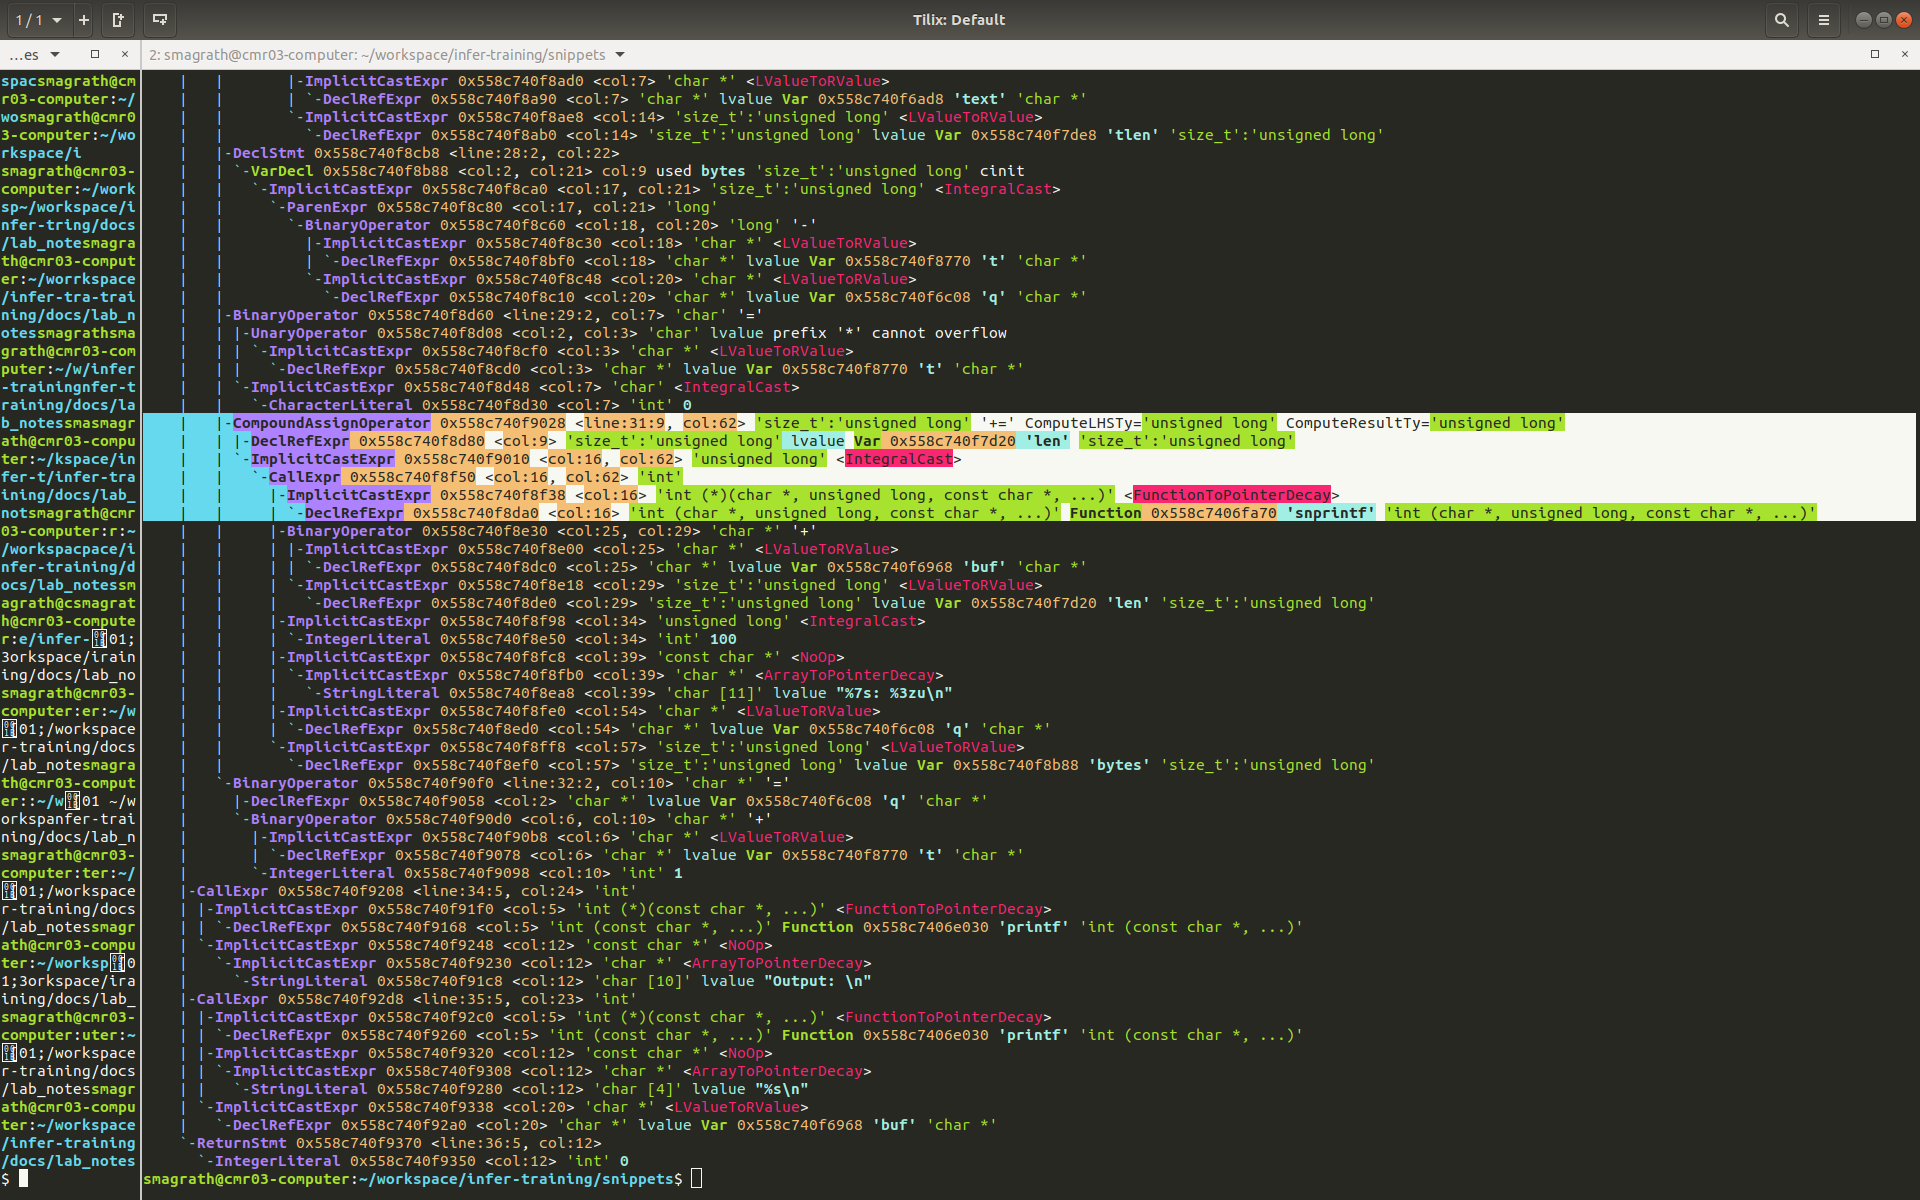
\includegraphics[width=\linewidth]{img/clang-ast}
	\caption[AST]{AST Screen shot}
	\label{fig:clang-ast}
\end{figure}

The next step is to specify a matching pattern that captures this syntactic structure.

\subsubsection{Step Two: Writing the Linter in AL}

There are various ways of writing this linter. 
We are going to write a simple version that over-approximates. That is, it can (and does) raise 
false positives. A more precise linter could be written but as we will see this has 
its own problems.

Add the following code to your \verb|mylinter.al| file.

\begin{verbatim}

DEFINE-CHECKER UNSAFE_SNPRINTF_ACCUMMULATION = {
    LET issnprintf = call_function(REGEXP("\\bsnprintf"));
    LET isaccum = is_node("CompoundAssignOperator");
    SET report_when = 
        issnprintf AND isaccum
    HOLDS-EVENTUALLY;
    SET message = "Possible Unsafe pointer accummulation using snprintf()";
    SET suggestion = "See Reference - TODO";
    SET severity = "ERROR";
};
\end{verbatim}

Note the following:
\begin{enumerate}
	\item We identify the \verb|snprintf| function using an AL \textit{predicate} called
	\verb|call_function|. This selects function call nodes in the AST. We further filter
	using a regular expression.
	\item We specifically select for \verb|CompoundAssignOperator| nodes in the AST.
	\item The particular tree pattern we want is where the call function is a child 
	of the \verb|CompoundAssignOperator| node. We can do this with the \verb|HOLDS-EVENTUALLY|
	CTL operator. Refer to the "AL Formulas" section of\\
	 \verb|https://fbinfer.com/docs/linters.html|. 
	In practice when developing linters you will need to become proficient with these formulas
	and linter debugging.
	\item Is this pattern completely correct to catch the bug we are after?	
\end{enumerate}

\exercise{Part Two: Linting for Unsafe Pointer Accumulation}

\begin{enumerate}
	\item Use Infer with the updated linter file for the code snippet.\\
	Verify that it identifies the problem line in the bug snippet.\\
	\verb|# infer run --linters-def-file ../mylinter.al -- clang -Wall -o test_2 test_2.c|
	\item For each of the targets run the linter and examine the bug reports:\\
	\verb|# infer run --keep-going --linters-only --linters-def-file ../mylinter.al -- make|
	\item You should find instances of false and true positives.\\ 
	Can you explain why the false positive occurred? 
	\item What are the limits of linting? Could you write a version of the \verb|snprintf()| bug 
	program that would not be caught by the linter?
\end{enumerate}

We are really only providing an introduction to Infer's linting capabilities here. 
You should examine the pre-provided linters that come with Infer to learn
more advanced and interesting examples. To find these linters simply \verb|grep -rn '*.al'|
in the Infer installation.

\subsection{Review}

What have we learnt so far?

\begin{itemize}
\item We learnt that linters are used to find syntactic bugs;
\item We have developed some simple linters using AL;
\item We have used Clang to generate AST information for code we are interested in;
\item We used the linters to find syntactic bugs in our targets.
\end{itemize}

\section{Final Notes}

The point of these lab notes is to give you an overview of Infer and some 
proficiency in using it to audit source code targets. You should develop
a sense of Infer's strengths and weaknesses and understand its place
amongst other tools for source code auditing. Static analysis is just one
useful technique for finding bugs in software. Being able to use Infer
well is an important and worthwhile skill to develop.

\subsection{Using Infer with CMake}

Getting Infer to work with the CMake build system can be difficult at first.
The basic approach is to get CMake to generate a compilation database
which Infer can then use.

\begin{enumerate}
	\item Edit the \verb|CmakeLists.txt| file to add the following:\\
	\verb|set(CMAKE_EXPORT_COMPILE_COMMANDS ON)|
	\item Run the CMake build:\\
	\verb|# CC=clang CXX=clang++ cmake -DCMAKE_EXPORT_COMPILE=1|\\
	This will export the JSON file  \verb|compile_commands.json|
	\item Run the following commands:\\
	\verb|# infer capture -- make|\\
	\verb|# infer analyze|\\
	\verb|# infer explore --html|\\
	Note: The Infer "run" mode is simply the "capture \& analyze" modes;
	
\end{enumerate}

\subsection{Further Work}
\begin{itemize}
	\item How to write \textit{models} of functions for use by Infer;
	\item How to write custom \textit{checkers} in OCaml for use in Infer;
	\item How to build Infer from source;
	\item How to integrate into a continuous integration pipeline;
	\item Microsoft builds.
\end{itemize}
